
% 
%%%%%%%%%%%%%%%%%%%%%%%%%%%%%%%%%%%%%%%%%
% Modification Log:
% Generated by Shengnan Liu on 21-01-2016
% Cleaned up for further usage on 10-06-2016
%%%%%%%%%%%%%%%%%%%%%%%%%%%%%%%%%%%%%%%%%
\documentclass[12pt, a4paper]{article}

\usepackage{adjustbox} % for minipage to the right

\usepackage{tabularx} % for resizebox?
\usepackage{graphicx}
%\usepackage{CJKutf8} % by pdfLaTeX, not LuaLaTeX
% *** https://www.math.sinica.edu.tw/www/tex/default14.jsp
\usepackage{xeCJK} % for Chinese, compiling by XeLaTex

\usepackage{fontspec} %設定字體
% Fandol font (the default)  not shown "內"
\setCJKmainfont{cwTeXHeiBold} %AR PL UMing TW MBE} % AR PL UMing TW MBE or "UKai" https://www.overleaf.com/learn/latex/Questions/Which_OTF_or_TTF_fonts_are_supported_via_fontspec%3F#Chinese
%BiauKai} %標楷體 from macOS %設定中文為系統上的字型,而英文不去更動,使用原TeX字型
% 微軟正黑體:Microsoft JhengHei 
%\XeTeXlinebreaklocale "zh"
%\XeTeXlinebreakskip = 0pt plus 1pt %這兩行一定要加,中文才能自動換行

\usepackage{outlines}
%\usepackage{booktabs}
% for tikz and gantt

\usepackage{multicol} % 
%\usepackage{animate}  % animation
%\usepackage{amsmath,amsfonts,amssymb} % This makes the equations appears better 

\usepackage{longtable}
\usepackage{xltabular} % the xltabular environment, which brings the functionalities of longtable to tabularx
\usepackage{array} % for centering or raggedleft
\newcolumntype{Z}{>{\raggedleft\let\newline\\\arraybackslash\hspace{0pt}}X}

\usepackage[table,xcdraw]{xcolor}

% https://github.com/AxelKrypton/genogram/blob/master/genogram_manual.pdf
\usepackage{genogram}

\begin{document}
%\maketitle

%\begin{abstract}
%Your abstract.
%\end{abstract}

%\section{Introduction}

\includegraphics[width=12cm]{logo_TMUH.jpg}

%Holistic 特別的我、須要特別的你---全人牙科臨床應用教案\\
\hspace{2.5cm} \Huge 全人關懷-實踐工作坊\\

\hspace{1.5cm} \large 全人醫療「8162北醫有愛 \hspace{0.4mm} 動心回饋」徵文辦法\\

%\hspace{0.3cm} \normalsize 投稿格式: \hspace{7.3cm} \today\\
%\date[today]{\today}

% Please add the following required packages to your document preamble:
% \usepackage{graphicx}
\begin{xltabular}{1.0\linewidth}[c]{|p{1.3cm}|p{4.4cm}|p{1.3cm}|p{4.4cm}|}
%\begin{xltabular}[ht]
%\centering
%\resizebox{0.9\textwidth}{!}{%
%\begin{tabular}{|l|l|l|l|}
\hline
主題 & \multicolumn{3}{l|}{張爺爺的顧慮}               \\ \hline
姓名 & 祁力行              & 員編       & 202029      \\ \hline
單位 & 牙科部口腔顎面外科        & 職稱       & 主治醫師        \\ \hline
內容 & \multicolumn{3}{l|}{(1000字以內,12號字,微軟正黑體)} \\ \hline

%\multicolumn{4}{|l|}{


%}
%    \\ \hline
%\multicolumn{4}{|l|}{}                         \\ \hline
%\end{tabular}%
%}
\end{xltabular}


% main text of story
張爺爺自40歲開始喝酒、吸菸,一天10支。60歲同時戒酒、戒菸。
張爺爺在78歲時,一週之內相繼確診為口腔癌(齒齦,第一期),膀胱癌(第一期)。
「爺爺,我們有很好的口腔癌手術團隊,拿掉癌細胞、下巴骨頭重建後,我們會陪著你一起復健,慢慢恢復吃東西、晨跑」,完成兩個癌症的分期與必要的檢查、會診之後,
因為膀胱癌的治療不複雜,我們建議張爺爺,迅速在北醫附醫接受膀胱鏡治療,術後追蹤使用「卡介苗沖洗膀胱」的免疫療法,然後就要掌握時機,接著進行口腔癌的治療。

一個月後,完成膀胱癌,接下來面對口腔癌。有過膀胱內視鏡(微創手術)的經驗,鄭爺爺非常害怕動手術,心中覺得,口腔癌若也能不用「開大刀」有多好。
出國留學、長年定居工作在美國的張家兒子,在網路上找到高雄某家口腔癌治療診所,話題就此轉到「動脈化療不必動刀,專治口腔癌」。不必開刀的吸引力太大。請原轉診醫師(他們熟識多年)幫忙勸說,也不成。
張爺爺堅定了不要開刀的決心,毅然赴高雄,接受陳醫師執行的自費動脈化療。
其實那並不是全世界主流的口腔癌療法,甚至是十年前被淘汰的方法,因為效果不明顯,而有腦部血管栓塞的風險。
%追蹤至 2020/07 
張爺爺和張奶奶非常信任附醫口腔外科,不定期會來門診追蹤,甚至應陳醫師的請求,安排電腦斷層與正子掃描,看看治療成效。為期一年,其實每次觀察口內牙齦癌症的情況,幾乎都沒有改變,更沒有長大或消失。
結束動脈化療與免疫藥物之後,陳醫師告訴張爺爺「治療結束,腫瘤仍在,接下來回去臺北的醫院中心,做放射治療吧」。

三個月後,進入過年期間,傳簡訊去問安「張爺爺晚安,放射治療很辛苦,請您一定要撐住。預祝農曆新年快樂。北醫 力行敬上」。
張爺爺是化學廠負責人,自上一代接手之後,已經工作五十年。來門診時再度提醒 「要避免膀胱癌,除了染髮劑,您的化學工廠更需要留心:減少接觸致癌化學藥品,工作人員,需配戴口罩與手套。多喝水降低毒素在體內的濃度,而憋尿會積累毒素,傷害膀胱。建議要多吃蔬菜水果,有助於解毒預防膀胱癌。」

完成放射治療,邁入80歲的張爺爺,體力恢復良好,也認為口腔癌已消失。
因為新冠病毒疫情起來,年長的張爺爺也暫時不敢來門診追蹤。
%2021/02 在新光醫院完成 radiation therapy (估算為 5000 cGy)。
完成放射治療半年後,疫情趨緩,
張爺爺來北醫附醫門診,因為診所醫師擔心他的牙根有個小腫塊,不太像「牙周病」造成的問題。經過電腦斷層、正子掃描與病理切片,證實了牙齦的癌細胞,繼續漫延。
「謝謝張爺爺。真的很擔心您,也很榮幸您回來找我們,請讓我們找一個最好的方法來幫助您。那癌細胞,其實從來沒有消失過,現在已經向著底下的骨頭,深深鑽進去。我可以看見它們。」
「趁一切來得及,請讓我們幫助您,是時候了,」
張爺爺問「上個週末開始,覺得下嘴唇麻木,牙齦都不會疼、不像兩年前一樣會流血」
「爺爺,因為下巴骨頭被腫瘤入侵,嘴唇的神經被破壞了,所以會麻,而反而不會疼」

此時,張家兒子在美國得知,接受美國醫師友人的建議,再度建議父親去某醫學中心,試試光動力療法。
張家奶奶說,「兒子心疼父親,就是想盡辦法不讓父親開刀。二年過去了,在高雄診所花費了很多很多錢,回臺北也做了放射治療,結果都沒有效。」
「啊,好辛苦,也好失望對不對?」
「光動力療法,僅限黏膜表層的癌細胞。因為雷射光照深度有限(最多一公分深),而張爺爺的癌細胞,深入下顎骨至少二公分,不僅無法清除癌細胞,更會引起顎骨壞死、潰爛,非常痛苦」

% the end
以病人為中心的生理、心理、靈性與社會之醫療照護,本著「關係在醫療以先」,取得信賴,全方面評估靈性和心理須求,再來替患者量身打造照護計畫。
%;於2)治療過程中除了緩解其生理不適外,同時能提前聚焦提升其自身復原力(Resilience)及自我價值感,以3)建立病後生活之正向期待和生活品質。



張爺爺必須面對「只剩下手術能夠治療」的現狀。我們做檢查的同時,也一再明確指出「目前除了手術,已經沒有別的方式可以痊癒」。
爺爺一直逃避無法下決心。在與張家兒子取得email聯繫後,
「請問父親不願意手術,真正害怕擔心是?我們需要召開家庭會議,集合手術切除、重建醫師團隊,來向你及父親母親,說明,手術後復原情況。」
「我們有很好的手術團隊,我們會陪著張爺爺一起復健,慢慢恢復吃東西、晨跑。
請不要再誤,已經過二年無效的治療,癌細胞進入骨頭後,會加速生長,到處漫延,終究連手術也無法進行。」
「請好好說服父親,不要再延宕手術治療的時機,太遲就很糟糕了。」
「面對非主流『替代療法』之原則:
第一是安全,第二是能有效清除癌細胞,且需要合法合理。」

面對病患的堅持與自主權,我們其實在關心與陪伴之餘,還要想辦法「入心」。
身心靈,社會(家庭)關係著癌症病患的一切,非常重要。
有關病患的恐懼、歉疚、社會關係,
仍不足需要努力。

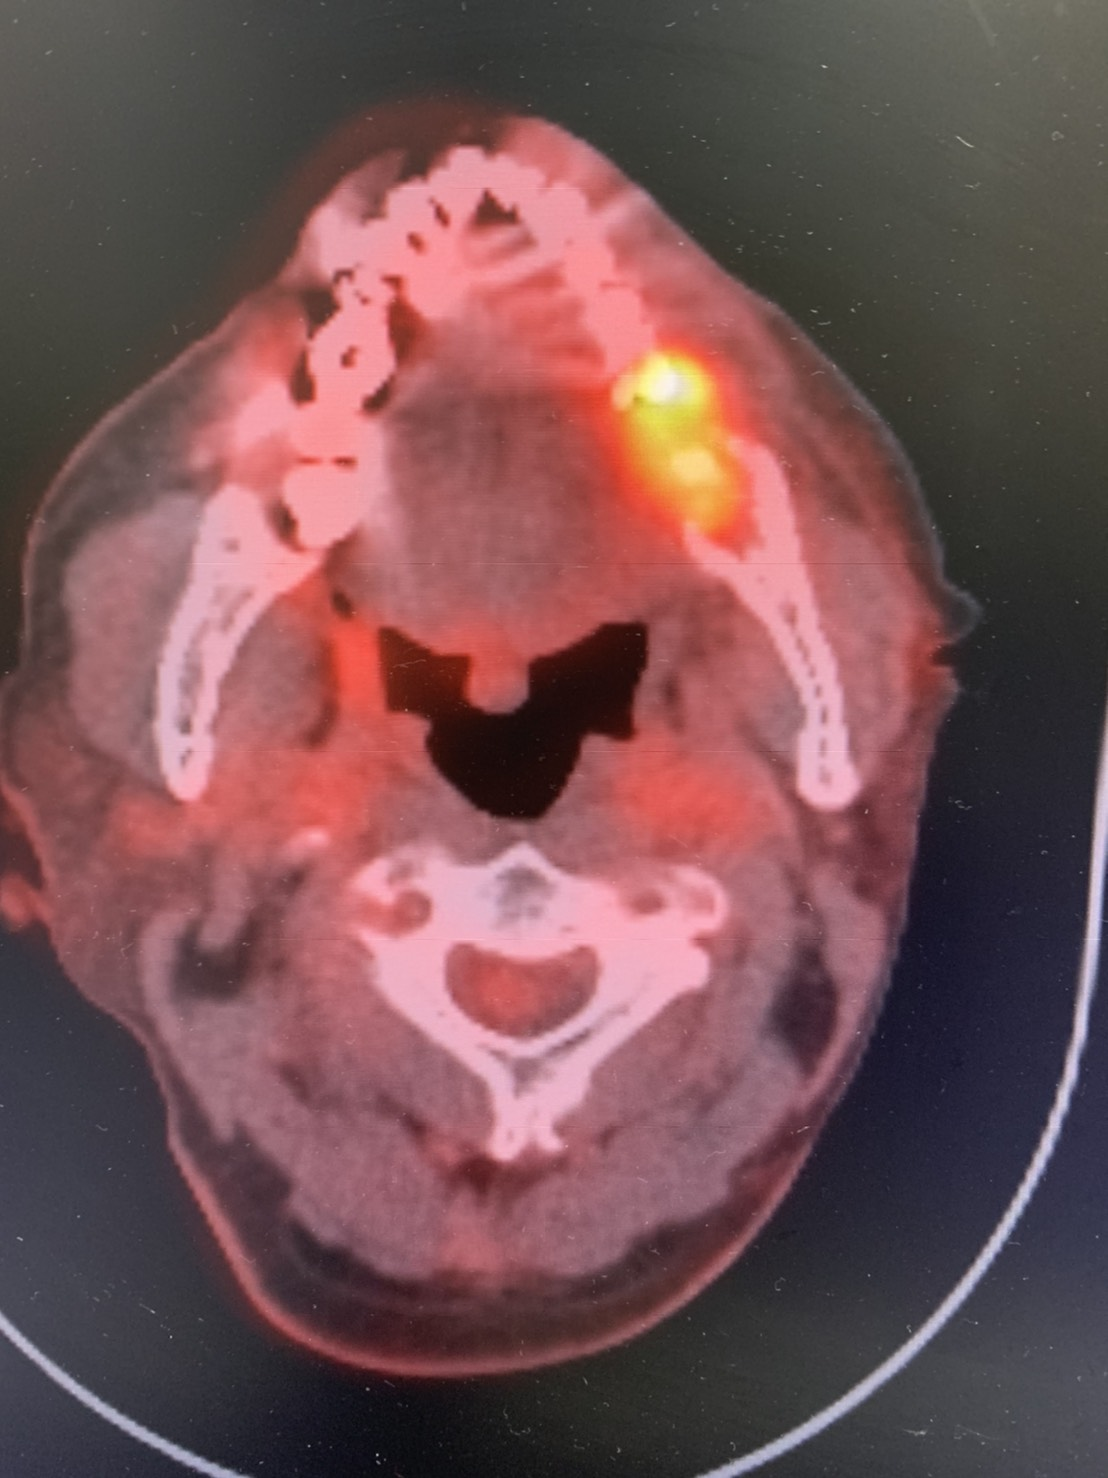
\includegraphics[width=10cm]{IMG_5873_PET_CT_scan_20210816.JPG}

\end{document}
% Please add the following required packages to your document preamble:
% \usepackage{longtable}
% Note: It may be necessary to compile the document several times to get a multi-page table to line up properly
%\begin{table}[]
%    \centering
%{\small\tabcolsep=3pt  % hold it local
%\setlength{\tabcolsep}{1pt}
%\setlength{\extrarowheight}{4pt}
\begin{xltabular}{1.0\linewidth}[c]{|p{2.3cm}|p{12.4cm}|l|} % tabularx + longtable
%\begin{longtable}[c]{\linewidth}{|l|l|l|}
\caption{}
\label{tab:my-table}\\
\hline
(空白) &
  內容 &
  備註 \\ \hline
\endfirsthead
%
%\multicolumn{3}{c}%
%{{\bfseries Table \thetable\ continued from previous page}} \\
%\endhead
%
Population; Patient &
  特別的我、須要特別的你\newline
%  ,須要輪椅輔助就診者‧\newline  
  ‧題目:牙科部 [次專科] 門診照護認知障礙與行動不便的病患\newline 
  ‧案例:Patient's profile \newline 
  1. Age:72 \newline 
  2. Gender:女 \newline 
  3. Occupation:家管 \newline 
  4. Genogram:如上圖 \newline 
  5. Hx.:高血壓、乳癌(十年前接受手術與放射治療)、思覺失調(Schizophrenia)、躁鬱症(bipolar disorder)、老年性失智 \newline 
  6. History of Present illness  \newline 
     來院方式:長女陪同輪椅前往牙科門診(近二年以來,接受牙科到宅服務,與次女同住)  \newline 
     CC:已經三個月沒有洗牙,覺得牙齒不乾淨(因為新冠病毐疫情,到宅牙醫暫停) \newline 
     PE:全口牙齒上沾滿食物,牙縫之間都是黃色牙結石  \newline 
     Lab data:腎功能稍差,其餘皆正常  \newline 
     Situation:病人以前很精明,家裡打理得很好,近十年來認為自己是太空裡的公主,雖然地球要被毀滅了,但大家必須放心,因為案主是將軍的後代,可以拯救案女。在家裡會自己緩慢走動,會自己開大門,但是無法下樓梯(無電梯的公寓四樓)。會幻聽幻想幻視。夜間不眠,大聲說話干擾到鄰居,並且會說大家都是壞人。\newline 
   &
  \\  \hline
Diagnosis; Intervention;\newline 
   Operation; Treatment Situation &
  1. 評估一般患者(案主)他/她們須要輪椅輔助的原因(主要診斷): 中樞神經問題 (老年性失智、血管性中風、頭部外傷、發育性疾患) 肢體問題 (肢體運動神經問題、外傷骨折、肌肉肌膜疼痛) 全身性急症 (耗弱、感染、疼痛、接受癌症治療中)\newline
  2. Epidemology for dental patient with special care:\newline
  人口老化情況嚴重下,老年牙醫學已是近年全球牙醫研究的主要趨勢,熟齡長者的口腔健康,帶來對健康的傷害恐怕更需要重視。\newline
    世界衛生組織(WHO)於2001年提出8020計畫,希望80歲的長者至少要能保存20顆以上的自然牙齒;行政院衛生福利部國民健康署曾做過統計,國內65歲以上的老年人,口內牙齒數仍保有24顆牙齒的僅有約4成左右,全口無牙的盛行率則有2成5以上。\newline
  3. 本案例病患因為老年性失智,在就醫過程中,行動不便,容易跌倒,上下輪椅須要攙扶,尚不須要被抱舉。候診時,會想去上洗手間。她的思覺失調(Schizophrenia)、躁鬱症(bipolar disorder)在藥物控制穩定期間,才能順利到醫院就診。\newline 
  4. 老年性失智症患者的後續照護需求:常有顏面及口腔疼痛、自我口腔、身體清潔不易(不能夠、不理解,或者是手部不方便)。 &
   \\ \hline
Holistic \newline
Assessment &
  {\color[HTML]{C0C0C0}說明:以上族群已有生理狀態之不便,須進一步評估其心理、靈性與社會之需求(請參考TMS 【國健署課程2/3】從安寧照護學全人心理層面)}\newline 
  心理需求:\newline
   在就醫路途中,及治療過程裡,緊張恐懼和焦慮,負面情緒的展現,甚至遵從意願降低、睡眠不佳、憂慮、易怒、自卑、挫折、恐慌、沒有等侯的耐心等。甚至要特別注意「因為是失能者,所以要求特別對待、優先看診」的心理狀態。\newline 
  {\color[HTML]{C0C0C0} (註記:處於心理狀態不穩定時,對於疼痛的解讀會有特別的表現,須多加留心。請參考TMS 【國健署課程3/3】從安寧照護學全人靈性層面:生命的意義與價值、愛與被愛、饒恕與被饒恕、與至高者的關係、盼望)}\newline
  靈性需求:\newline
  就醫過程中被接納、被同理的需求、受到尊重的對待、對於治療之期待,因為焦慮而產生「很多的疑問」,念頭反覆在同一個陷井裡打轉,有時滿腦子的疑問卻不敢問醫生(怕佔用太多時間),難以下決定。另外一個層面是,如果認知功能已經受損,有時在門診不易評估「是否聽得懂」,無聲的靈性須求得轉向陪伴的家屬。\newline 
  {\color[HTML]{C0C0C0}(請參考TMS【國健署課程1/3】從安寧照護學全人社會層面)}\newline 
  社會需求:
   因疾病及就醫所產生社會角色改變,病後生活及工作影響、家屬的支持、家庭權力結構轉移、社會資源需求(例如:職災給付、長照2.0服務)或需通報之社會議題等。 陪伴的家屬,與外籍看護,代表對患者的最主要的支持。有時會擔心趕不上「復康巴士」的約定接送時間。{\color[HTML]{C0C0C0}(註記:以病人為先,重視其有聲與無聲之表現,例如頻頻看手錶。) } &
   \\ \hline
Major Finding &
  {\color[HTML]{C0C0C0}(說明:根據上述族群、診斷情境的評估)}\newline 
   牙科部 [次專科] 於臨床醫療照護中,與案主及女兒所期望的不同,\newline 
   醫療方面: 醫師無法完全了解患者的主訴(因為她說不明白),同住女兒(次女)亦不容易掌握到案主最急迫的問題,必須耐心傾聽,處處提問。案主有全身性慢性疾病,血壓、血栓、雙磷酸鹽類藥物,腎功能,這些對口腔健康的影響很大,故她的治療計畫必須量身打造。\newline 
   非醫療方面: 不易掌握適合案主的刷牙方式。案主就診時,因為診間冷氣很強,她手腳冰冷、想去洗手間,都不敢說。 &
   \\ \hline
Establishing; Modifying SOP or Intervention for a better Holistic Care &
  {\color[HTML]{C0C0C0}(說明:針對前項的改善方式,以達成促進健康與預防疾病。適當提醒長期照護或安寧照護)} \newline 
  醫療方面: 一般針對中風/認知功能不足的情況,可設法了解與判斷患者的主訴,與家屬現場討論,找出最急迫的問題,訂定簡化版的牙科治療計劃。 備齊各科就診病歷、報告與數據(例如血糖、血壓、血栓、癌症用藥,放射治療、雙磷酸鹽類藥物,免疫療法,肝腎功能),整理摘要,在病歷紀錄慢性病的目前概況,以及未來對口腔健康可能的不利影響,必訂定因應方案,與正確衛教。使用簡短、清楚、而且是患者能夠聽懂的話語手勢。\newline 
   以本案主為例,曾經是乳癌患者
   %正在住院接受化療治療,因為黏膜潰瘍、牙齦腫脹,會診牙科 [次專科] 時坐輪椅就診,全口 panoramic x-ray\newline 現階段口腔清潔的方式(因應潰瘍疼痛刷牙困難)必然可以撐過這個階段。更要
%   評估過後,除了
% (其實是在簡單暗示,日後若必須使用雙磷酸鹽類時,已有良好的口腔健康狀態,才能順利接受藥物,以免下顎骨的併發症)
   我們安排超音波洗牙(門診或到宅),指導口腔清潔的方式(用她能聽懂、可以做到的方式),適時鼓勵,強調保持良好口腔清潔習慣的重要性,定期(三個月)於牙科追蹤,因為她曾經使用過雙磷酸鹽類藥物,要極力保持良好的口腔健康狀態,避免下顎骨受損的併發症(medication-related osteonecrosis of jaw, MRONJ)。\newline 
   非醫療方面: 掌握失能對其自我照顧的方法,請家屬下一次帶著他的牙刷,並且準備牙線棒與牙間刷(最小號),於門診時請她自己刷一次,然後醫師示範教給案長女、案次女(她們沒有僱請外籍照護工)幫案主再刷一次(補強)。留心觀察患者的手指協調能力,以及視力。 &
   \\ \hline
Expected Outcomes &
  {\color[HTML]{C0C0C0}(說明:預期之成效與其評估的方式)}\newline 
   醫療方面: 落實「減法策略」,以期減少患者的感染風險、減少家屬、外籍看護工的照顧壓力。由患者的發燒、住院、肺炎的次數可以評估其成效。輔以病患家屬的滿意度調查。 就診時接上血壓計,隨時量測生命徵象(包括疼痛),並於病歷中詳實紀錄,預估對口腔健康可能的不利影響,並訂定因應方案。\newline 
   非醫療方面: 預期成效是,能落實照顧者對患者的口腔清潔。評估方式是,回診時檢查塗上「牙菌斑顯示劑」染色。不必問候「會不會冷、想不想去上洗手間」,患者會自行說出須求。 &
   \\ \hline
Take-home messages &
    1. 病患的心理、社會及靈性需求能被滿足,回過頭來處理生理、病情才能事半功倍\newline
    2. 醫者只要靜下心來,人人都能充份扮演好「靈性諮商員」的角色\newline
    3. 萬芳醫院牙科部 [次專科]  的全人照護專案,也正在規畫階段 \newline
    &
   \\ \hline
\end{xltabular}

%\end{longtable}



